% tex file for convolution
\subsubsection{Convolution}
\par \indent As our study is structured around event-related neurological 
stimulus and not block stimulus as was discussed in class, a similar 
approach to representing the hemodynamic response could not be done. 

The general assumption is that there is a relationship between the 
hemodynamic response to neurological stimulation, where a single 
stimulation generates a delayed hemodyamic response that mirrors 
a double gamma function, and that there is a natural linear/additive 
nature when there are multiple stimulations one just adds the response 
functions started at different times, as defined below:

\begin{equation} \label{eq:convolve}
r(t)= \sum_{i=1}^n \psi_{i} \phi_{i}(t-t_i)
\end{equation}

\noindent where $\psi$ is the amplitude of the response stimulus (always $1$ 
in our case), and $\phi_{i}$ is the hemodynamic response started at the $i$th 
stimulation ($t_i$).

The five approaches we attempted can be divided into three subcategories: 
\textbf{(1)} a strict replication of equation \ref{eq:convolve}; \textbf{(2)} 
a similar function as \textbf{(1)} that utilizes matrix multiplication; and 
\textbf{(3)} a function that splits the intervals between each scan (two 
seconds) into a certain number of even slices, then puts the stimulus into the 
closest split, using \texttt{np.convolve} on this stimulus and a detailed hrf 
function, and then reducing the output back into the two-second time intervals. 
Detailed exploration of this matter can be found in the Appendix \ref{app_convolution}.

We compared these methods based on accuracy and speed. Figure 
\ref{fig:convolution_a} displaces accuracy comparison, and the table in 
Table~\ref{fig:convolution_a} show the accuracy based off of 
\texttt{ipython}'s \texttt{timeit} function.



\begin{figure}[ht]
\centering
	\begin{minipage}[b]{0.45\linewidth}
		\centering
		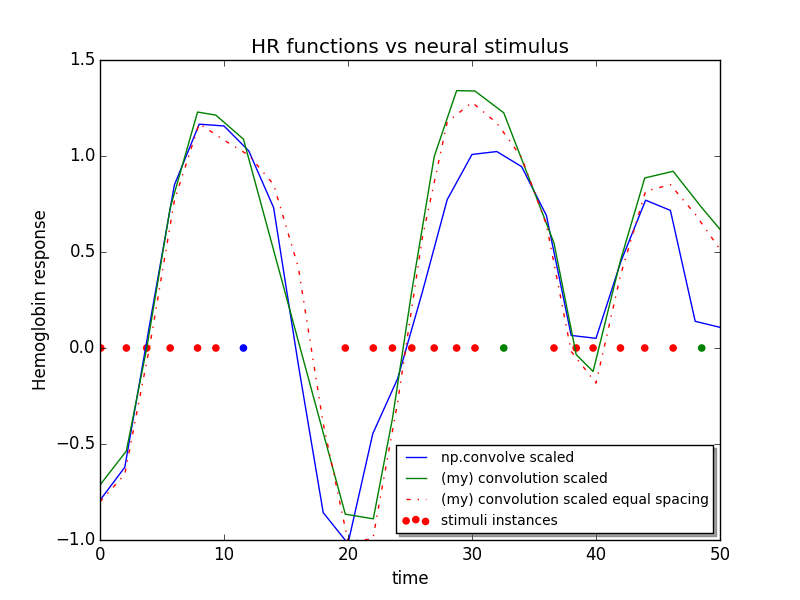
\includegraphics[width=.8\linewidth]{../images/convolution_vs_neural_stimulus}
		% needs to be from the event_related_HRF_script2.py 
		\caption{\scriptsize{Different convolution functions vs. the Neural stimulus}}
		\label{fig:convolution_a}

	\end{minipage}
\quad
	\begin{minipage}[b]{0.45\linewidth}
		\centering
		\begin{tabular}{|l | c|}
		\hline
		name in graph       & Speed per loop \\
		\hline
		np naive approach & 14.4 $\mu$s  \\
		user 2     		    & 972 ms  \\
		user 3     		    & 1.15 s    \\
		user 4 (15 cuts)      & 98.3 ms \\
		user 4 (30 cuts)      & 185 ms  \\
		user 5     	 	    & 110 ms   \\
		\hline
		\end{tabular}
		\vspace{5mm}
		\label{tab:convolution_a}
		\captionof{table}{\scriptsize{Speed to create HRF predictions for 
		Subject 001, all conditions}}
	\end{minipage}
\end{figure}

\par \noindent The first method in the table ``np naive approach'' blindly 
plugs in our data into the \texttt{np.convolve} function. It is provided to 
showcase potential speed. The failure of the "np naive approach" was the 
motivating factor behind the rest of the hemodynamic response convolution 
analysis, due to a lack of equidistant spacing of stimulus and scans. The 
``user 2'' and ``user 3'' runs fall under subcategory 
\textbf{(1)}. The ``user 2'' was the first approach to
match the theory, but it matches the stimulation times and not the scan times.
The ``user 3'' is the most theoretically sound model (and is our standard for 
accuracy). The ``user 5'' falls under subcategory \textbf{(2)}, ``User 5''  is
our matrix version of the theory, and has the same accuracy as ``user 3''. The 
``user 4'' models falls under subcategory \textbf{(3)}, the methods that use the
grid cut usage of \texttt{np.convolve} with notations for the number of slices 
between each scan. We concluded that "user 4 (15 cuts)" was the best approach 
since it gives us speed and very close accuracy to the golden standard - ``user 
3".

\subsubsection{Time Correction}

\par \indent The fMRI machine scans each voxel at a slightly different time. 
In our case, the lowest horizontal slice was scanned first, with the later 
scans moving progressively toward the top of the brain. The signs of this 
linear change in time of scan was observed when running simple regression on 
the data and the hemodyamic response beta values from all conditions grouped 
together. We corrected for this  by shifting the times of stimulus 
``backwards'' for voxels scanned later to directly correct for the delay of 
the scan (assuming that each layer of the scan took 2/34 of a second).

\subsubsection{Multiple Conditions}

\par \indent Originally we used multiple regression to take into account the 
three different types of stimulus (pump, explode, cash-out) to see if the 
separation of these stimuli can better describe the response. We did this by 
creating separate predicted hemodynamic reponses for each to allow for 
different amplitudes for each type of condition. As will be noted in the 
\textit{Model selection} [\ref{model_selection}] portion later, we did not 
observe a large difference in
the results values we obtained, so we did not continue with this exploration. 
In figure \ref{fig:all_cond_time}, we can see the different conditions broken 
up.


\begin{figure}[ht]
\centering
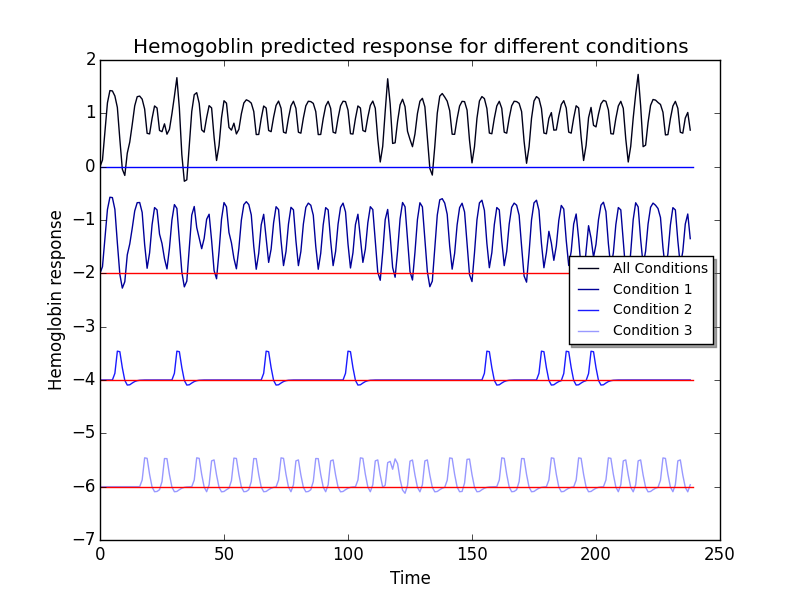
\includegraphics[scale=.5]{../images/all_cond_time}  
\caption{Plotting all predicted HR for conditions.}
\label{fig:all_cond_time}
\end{figure}

A more detailed discussion about our approach and theory behind convolution 
of the hemodynamic response with the neurological response can be found 
in the Appendix on Convolution \ref{app_convolution}.

